\documentclass[11pt]{scrartcl}
\usepackage{polski}
\usepackage[polish]{babel}

\usepackage{graphicx, float, caption, subcaption}
\usepackage{amsmath}
\usepackage{tabularx}
\graphicspath{{images/}}

\title{Laboratorium 1 - Predykaty geometryczne}
\author{Mateusz Podmokły}
\date{18 październik 2023}

\begin{document}
    \maketitle
    \section{Specyfikacja użytego środowiska}

    Specyfikacja:

    \begin{itemize}
        \item Środowisko: Jupyter Notebook,
        \item Język programowania: Python,
        \item System operacyjny: Microsoft Windows 11,
        \item Architektura systemu: x64.
    \end{itemize}
    \section{Przebieg ćwiczenia}

    Ćwiczenie polega na analizie wyników algorytmów obliczających na różne sposoby
    położenie punktów względem prostej.

    \subsection{Losowanie punktów}

    Wylosowane zostały następujące zbiory punktów:

    \begin{enumerate}
        \item \(10^5\) losowych punktów o współrzędnych z przedziału \([-1000,1000]\),
        \item \(10^5\) losowych punktów o współrzędnych z przedziału \([-10^{14},10^{14}]\),
        \item 1000 losowych punktów leżących na okręgu o środku \((0,0)\)
        i promieniu $R=100$,
        \item 1000 losowych punktów o współrzędnych z przedziału [-1000, 1000]
        leżących na prostej wyznaczonej przez wektor $\overrightarrow{ab}$, gdzie
        $a=(-1,0)$, $b=(1,\dfrac{1}{10})$.
    \end{enumerate}

    \begin{figure}[H]
        \centering
        \begin{minipage}{0.45\linewidth}
          \centering
          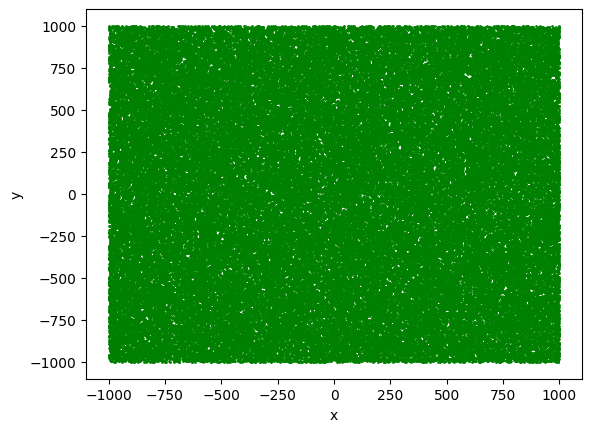
\includegraphics[width=1\linewidth]{1_1.png}
          \caption{Zbiór 1. - obszar kwadratowy.}
        \end{minipage}
        \begin{minipage}{0.45\linewidth}
          \centering
          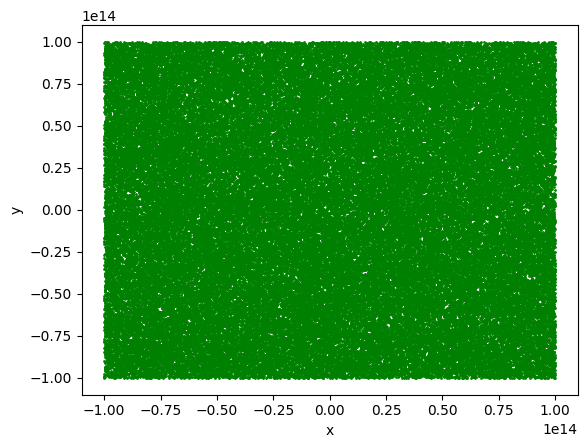
\includegraphics[width=1\linewidth]{1_2.png}
          \caption{Zbiór 2. - obszar kwadratowy.}
        \end{minipage}
    \end{figure}

    \begin{figure}[H]
        \centering
        \begin{minipage}{0.45\linewidth}
          \centering
          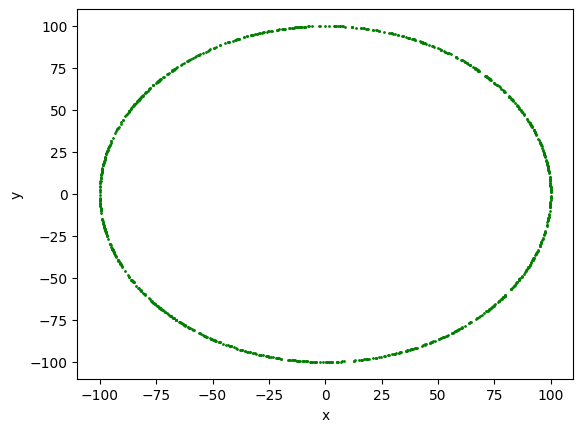
\includegraphics[width=1\linewidth]{1_3.png}
          \caption{Zbiór 3. - okrąg.}
        \end{minipage}
        \begin{minipage}{0.45\linewidth}
          \centering
          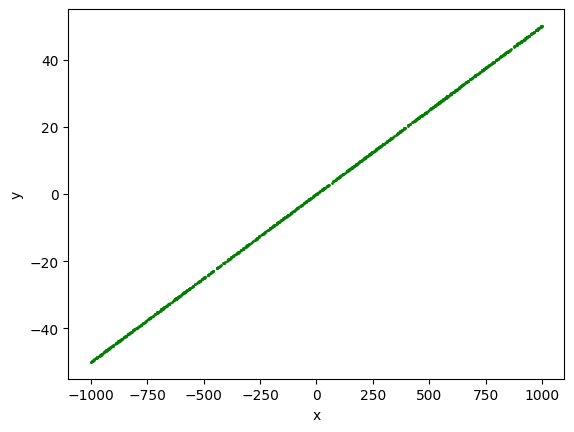
\includegraphics[width=1\linewidth]{1_4.png}
          \caption{Zbiór 4. - prosta.}
        \end{minipage}
    \end{figure}

    \subsection{Funkcje obliczające wyznacznik macierzy}
    Łatwo zbadać położenie punktu względem prostej obliczając wyznacznik macierzy
    2x2 lub 3x3. Jeżeli $det(a,b,c) > 0$ to punkt leży po lewej stronie prostej,
    $det(a,b,c) < 0$ - leży po prawej, a jeżeli $det(a,b,c) = 0$ to dany punkt
    leży na prostej. Dla prostej wyznaczonej przez wektor $\overrightarrow{ab}$
    i punktu $c$ mamy wyznacznik 2x2:

    \[det(a,b,c)=
    \begin{vmatrix}
        a_x - c_x & a_y - c_y \\
        b_x - c_x & b_y - c_y
    \end{vmatrix}
    =(a_x - c_x)(b_y - c_y) - (b_x - c_x)(a_y - c_y)\]
    oraz wyznacznik 3x3:

    \[det(a,b,c)=
    \begin{vmatrix}
        a_x & a_y & 1 \\
        b_x & b_y & 1 \\
        c_x & c_y & 1
    \end{vmatrix}
    =a_x b_y + a_y c_x + b_x c_y - c_x b_y - b_x a_y - a_x c_y\]
    Do testów użyta została funkcja obliczająca wyznacznik wbudowana w bibliotekę
    Numpy linalg.det() oraz własne implementacje.

    \subsection{Obliczanie klasyfikacji punktów z użyciem powyższych funkcji}
    Dla każdego zbioru obliczone zostały klasyfikacje punktów przy użyciu
    typu danych float64 oraz $\epsilon=10^{-12}$ na 4 sposoby:

    \begin{itemize}
        \item wyznacznik 2x2 zaimplementowany ręcznie,
        \item wyznacznik 2x2 z biblioteki Numpy,
        \item wyznacznik 3x3 zaimplementowany ręcznie,
        \item wyznacznik 3x3 z biblioteki Numpy.
    \end{itemize}
    Następnie obliczenia zostały powtórzone z użyciem $\epsilon=1$. Na koniec
    typ danych został ustawiony na float32 i wszystko ponownie przeliczone.
    Wyniki obliczeń zostaną przedstawione poniżej.
    \subsubsection*{}
    Przykładowe klasyfikacje punktów ze zbiorów:

    \begin{figure}[H]
        \centering
        \begin{minipage}{0.4\linewidth}
          \centering
          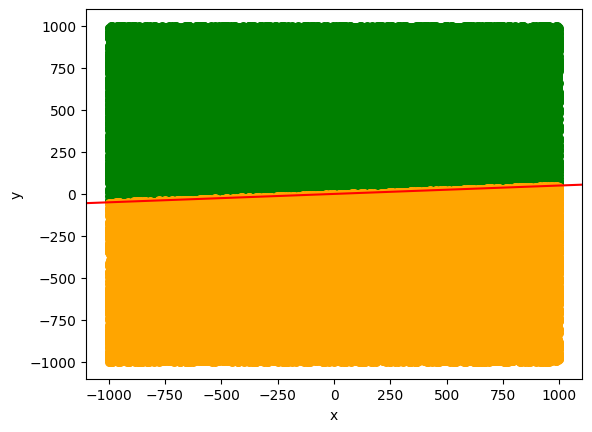
\includegraphics[width=1\linewidth]{1_5.png}
          \caption{Zbiór 1. - obszar kwadratowy.}
        \end{minipage}
        \begin{minipage}{0.4\linewidth}
          \centering
          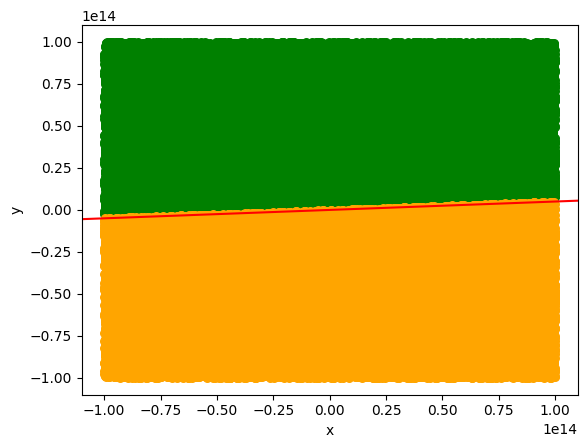
\includegraphics[width=1\linewidth]{1_6.png}
          \caption{Zbiór 2. - obszar kwadratowy.}
        \end{minipage}
    \end{figure}

    \begin{figure}[H]
        \centering
        \begin{minipage}{0.4\linewidth}
          \centering
          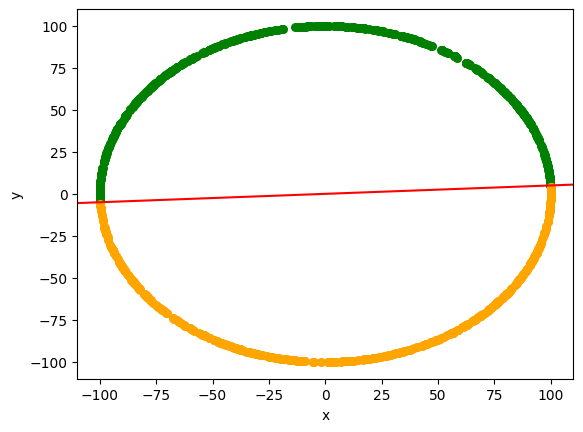
\includegraphics[width=1\linewidth]{1_7.png}
          \caption{Zbiór 3. - okrąg.}
        \end{minipage}
        \begin{minipage}{0.4\linewidth}
          \centering
          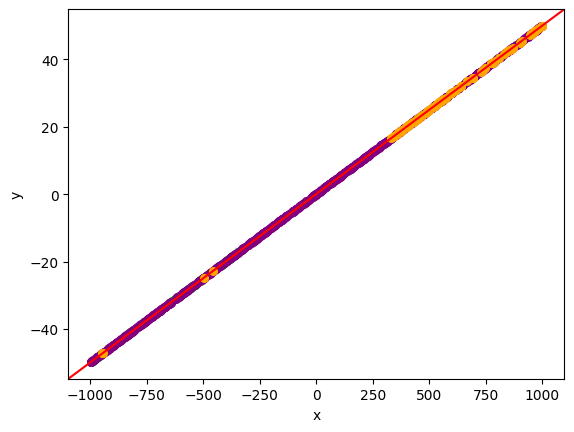
\includegraphics[width=1\linewidth]{1_8.png}
          \caption{Zbiór 4. - prosta.}
        \end{minipage}
    \end{figure}



    \section{Analiza wyników}
    \subsection{Zestawienie otrzymanych danych:}
    \subsubsection{Typ danych float64, $\epsilon=10^{-12}$}

    \begin{table}[H]
        \centering
        \renewcommand{\arraystretch}{1.5}
        \begin{tabular}{| c | c | c | c |}
            \hline
            & Po lewej & Po prawej & Na prostej \\
            \hline
            Zbiór 1 & 49979 & 50021 & 0 \\
            \hline
            Zbiór 2 & 50064 & 49927 & 9 \\
            \hline
            Zbiór 3 & 513 & 487 & 0 \\
            \hline
            Zbiór 4 & 80 & 94 & 826 \\
            \hline
        \end{tabular}
        \renewcommand{\arraystretch}{1.5}
        \caption{Wyznacznik 2x2 implementacja własna.}
    \end{table}
    \begin{table}[H]
        \centering
        \renewcommand{\arraystretch}{1.5}
        \begin{tabular}{| c | c | c | c |}
            \hline
            & Po lewej & Po prawej & Na prostej \\
            \hline
            Zbiór 1 & 49979 & 50021 & 0 \\
            \hline
            Zbiór 2 & 50063 & 49926 & 11 \\
            \hline
            Zbiór 3 & 513 & 487 & 0 \\
            \hline
            Zbiór 4 & 118 & 107 & 775 \\
            \hline
        \end{tabular}
        \renewcommand{\arraystretch}{1.5}
        \caption{Wyznacznik 2x2 Numpy.}
    \end{table}
    \begin{table}[H]
        \centering
        \renewcommand{\arraystretch}{1.5}
        \begin{tabular}{| c | c | c | c |}
            \hline
            & Po lewej & Po prawej & Na prostej \\
            \hline
            Zbiór 1 & 49979 & 50021 & 0 \\
            \hline
            Zbiór 2 & 50067 & 49933 & 0 \\
            \hline
            Zbiór 3 & 513 & 487 & 0 \\
            \hline
            Zbiór 4 & 0 & 0 & 1000 \\
            \hline
        \end{tabular}
        \renewcommand{\arraystretch}{1.5}
        \caption{Wyznacznik 3x3 implementacja własna.}
    \end{table}
    \begin{table}[H]
        \centering
        \renewcommand{\arraystretch}{1.5}
        \begin{tabular}{| c | c | c | c |}
            \hline
            & Po lewej & Po prawej & Na prostej \\
            \hline
            Zbiór 1 & 49979 & 50021 & 0 \\
            \hline
            Zbiór 2 & 50067 & 49933 & 0 \\
            \hline
            Zbiór 3 & 513 & 487 & 0 \\
            \hline
            Zbiór 4 & 0 & 0 & 1000 \\
            \hline
        \end{tabular}
        \renewcommand{\arraystretch}{1.5}
        \caption{Wyznacznik 3x3 Numpy.}
    \end{table}

    \subsubsection{Typ danych float64, $\epsilon=1$}
    \begin{table}[H]
        \centering
        \renewcommand{\arraystretch}{1.5}
        \begin{tabular}{| c | c | c | c |}
            \hline
            & Po lewej & Po prawej & Na prostej \\
            \hline
            Zbiór 1 & 49799 & 50153 & 48 \\
            \hline
            Zbiór 2 & 50047 & 49945 & 8 \\
            \hline
            Zbiór 3 & 476 & 519 & 5 \\
            \hline
            Zbiór 4 & 0 & 0 & 1000 \\
            \hline
        \end{tabular}
        \renewcommand{\arraystretch}{1.5}
        \caption{Wyznacznik 2x2 implementacja własna.}
    \end{table}
    \begin{table}[H]
        \centering
        \renewcommand{\arraystretch}{1.5}
        \begin{tabular}{| c | c | c | c |}
            \hline
            & Po lewej & Po prawej & Na prostej \\
            \hline
            Zbiór 1 & 49799 & 50153 & 48 \\
            \hline
            Zbiór 2 & 50045 & 49944 & 11 \\
            \hline
            Zbiór 3 & 476 & 519 & 5 \\
            \hline
            Zbiór 4 & 0 & 0 & 1000 \\
            \hline
        \end{tabular}
        \renewcommand{\arraystretch}{1.5}
        \caption{Wyznacznik 2x2 Numpy.}
    \end{table}
    \begin{table}[H]
        \centering
        \renewcommand{\arraystretch}{1.5}
        \begin{tabular}{| c | c | c | c |}
            \hline
            & Po lewej & Po prawej & Na prostej \\
            \hline
            Zbiór 1 & 49799 & 50153 & 48 \\
            \hline
            Zbiór 2 & 50049 & 49951 & 0 \\
            \hline
            Zbiór 3 & 476 & 519 & 5 \\
            \hline
            Zbiór 4 & 0 & 0 & 1000 \\
            \hline
        \end{tabular}
        \renewcommand{\arraystretch}{1.5}
        \caption{Wyznacznik 3x3 implementacja własna.}
    \end{table}
    \begin{table}[H]
        \centering
        \renewcommand{\arraystretch}{1.5}
        \begin{tabular}{| c | c | c | c |}
            \hline
            & Po lewej & Po prawej & Na prostej \\
            \hline
            Zbiór 1 & 49979 & 50153 & 48 \\
            \hline
            Zbiór 2 & 50049 & 49951 & 0 \\
            \hline
            Zbiór 3 & 476 & 519 & 5 \\
            \hline
            Zbiór 4 & 0 & 0 & 1000 \\
            \hline
        \end{tabular}
        \renewcommand{\arraystretch}{1.5}
        \caption{Wyznacznik 3x3 Numpy.}
    \end{table}

    \subsubsection{Typ danych float32, $\epsilon=10^{-12}$}
    \begin{table}[H]
        \centering
        \renewcommand{\arraystretch}{1.5}
        \begin{tabular}{| c | c | c | c |}
            \hline
            & Po lewej & Po prawej & Na prostej \\
            \hline
            Zbiór 1 & 50252 & 49748 & 0 \\
            \hline
            Zbiór 2 & 49986 & 50008 & 6 \\
            \hline
            Zbiór 3 & 531 & 469 & 0 \\
            \hline
            Zbiór 4 & 408 & 404 & 188 \\
            \hline
        \end{tabular}
        \renewcommand{\arraystretch}{1.5}
        \caption{Wyznacznik 2x2 implementacja własna.}
    \end{table}
    \begin{table}[H]
        \centering
        \renewcommand{\arraystretch}{1.5}
        \begin{tabular}{| c | c | c | c |}
            \hline
            & Po lewej & Po prawej & Na prostej \\
            \hline
            Zbiór 1 & 50252 & 49748 & 0 \\
            \hline
            Zbiór 2 & 49983 & 50008 & 11 \\
            \hline
            Zbiór 3 & 531 & 469 & 0 \\
            \hline
            Zbiór 4 & 429 & 427 & 144 \\
            \hline
        \end{tabular}
        \renewcommand{\arraystretch}{1.5}
        \caption{Wyznacznik 2x2 Numpy.}
    \end{table}
    \begin{table}[H]
        \centering
        \renewcommand{\arraystretch}{1.5}
        \begin{tabular}{| c | c | c | c |}
            \hline
            & Po lewej & Po prawej & Na prostej \\
            \hline
            Zbiór 1 & 50252 & 49748 & 0 \\
            \hline
            Zbiór 2 & 49990 & 50010 & 0 \\
            \hline
            Zbiór 3 & 531 & 469 & 0 \\
            \hline
            Zbiór 4 & 408 & 404 & 188 \\
            \hline
        \end{tabular}
        \renewcommand{\arraystretch}{1.5}
        \caption{Wyznacznik 3x3 implementacja własna.}
    \end{table}
    \begin{table}[H]
        \centering
        \renewcommand{\arraystretch}{1.5}
        \begin{tabular}{| c | c | c | c |}
            \hline
            & Po lewej & Po prawej & Na prostej \\
            \hline
            Zbiór 1 & 50252 & 49748 & 0 \\
            \hline
            Zbiór 2 & 49990 & 50010 & 0 \\
            \hline
            Zbiór 3 & 531 & 469 & 0 \\
            \hline
            Zbiór 4 & 408 & 404 & 188 \\
            \hline
        \end{tabular}
        \renewcommand{\arraystretch}{1.5}
        \caption{Wyznacznik 3x3 Numpy.}
    \end{table}
    
    \subsubsection{Typ danych float32, $\epsilon=1$}
    \begin{table}[H]
        \centering
        \renewcommand{\arraystretch}{1.5}
        \begin{tabular}{| c | c | c | c |}
            \hline
            & Po lewej & Po prawej & Na prostej \\
            \hline
            Zbiór 1 & 49998 & 49946 & 56 \\
            \hline
            Zbiór 2 & 50147 & 49847 & 6 \\
            \hline
            Zbiór 3 & 499 & 496 & 5 \\
            \hline
            Zbiór 4 & 0 & 0 & 1000 \\
            \hline
        \end{tabular}
        \renewcommand{\arraystretch}{1.5}
        \caption{Wyznacznik 2x2 implementacja własna.}
    \end{table}
    \begin{table}[H]
        \centering
        \renewcommand{\arraystretch}{1.5}
        \begin{tabular}{| c | c | c | c |}
            \hline
            & Po lewej & Po prawej & Na prostej \\
            \hline
            Zbiór 1 & 49998 & 49946 & 56 \\
            \hline
            Zbiór 2 & 50147 & 49849 & 4 \\
            \hline
            Zbiór 3 & 499 & 496 & 5 \\
            \hline
            Zbiór 4 & 0 & 0 & 1000 \\
            \hline
        \end{tabular}
        \renewcommand{\arraystretch}{1.5}
        \caption{Wyznacznik 2x2 Numpy.}
    \end{table}
    \begin{table}[H]
        \centering
        \renewcommand{\arraystretch}{1.5}
        \begin{tabular}{| c | c | c | c |}
            \hline
            & Po lewej & Po prawej & Na prostej \\
            \hline
            Zbiór 1 & 49998 & 49946 & 56 \\
            \hline
            Zbiór 2 & 50151 & 49849 & 0 \\
            \hline
            Zbiór 3 & 499 & 496 & 5 \\
            \hline
            Zbiór 4 & 0 & 0 & 1000 \\
            \hline
        \end{tabular}
        \renewcommand{\arraystretch}{1.5}
        \caption{Wyznacznik 3x3 implementacja własna.}
    \end{table}
    \begin{table}[H]
        \centering
        \renewcommand{\arraystretch}{1.5}
        \begin{tabular}{| c | c | c | c |}
            \hline
            & Po lewej & Po prawej & Na prostej \\
            \hline
            Zbiór 1 & 49998 & 49946 & 56 \\
            \hline
            Zbiór 2 & 50151 & 49849 & 0 \\
            \hline
            Zbiór 3 & 499 & 496 & 5 \\
            \hline
            Zbiór 4 & 0 & 0 & 1000 \\
            \hline
        \end{tabular}
        \renewcommand{\arraystretch}{1.5}
        \caption{Wyznacznik 3x3 Numpy.}
    \end{table}

    \subsection{Analiza otrzymanych danych}
    Można zauważyć że liczby punktów po prawej i po lewej stronie prostej są
    do siebie zbliżone. Wyznacznik 3x3 znajduje mniej punktów na prostej
    niż wyznacznik 2x2 (Tabela 1 i 3), nastomiast ręcznie zaimplementowane
    wyznaczniki więcej w porównaniu do bibliotecznych (Tabela 10 i 11). Po zwiększeniu tolerancji
    dla zera znacznie wzrasta liczba punktów klasyfikowanych jako leżące na
    prostej. Natomiast zmiana precyzji z float64 na float32, która zmniejsza
    dokładność obliczeń, powoduje, że wiele punktów ze zbioru 4. leżących na
    prostej jest błędnie klasyfikowane jako nieleżące na prostej.

    \section{Wnioski}
    \subsection*{Wyznaczniki}
    Mniejsza liczba punktów klasyfikowanych przez wyznacznik 3x3 jako leżące
    na prostej może być spowodowana większą liczbą mnożeń niż w przypadku
    wyznacznika 2x2 co powoduje zaokrąglenia wyników i straty w dokładności.
    Podobnie może być w przypadku różnic między wyznacznikiem zaimplementowanym
    ręcznie, a wersją pochodzącą z biblioteki Numpy - druga funkcja jest
    przystosowana do obliczania dowolnych wyznaczników $n$ x $n$, więc ilość
    obliczeń, które są przeprowadzane na danych wejściowych może być znacznie
    większa niż wewnąrtrz funkcji zaimplementowanych ręcznie, służących do
    obliczania konkretnego rodzaju wyznacznika. Nadmierne obliczenia mogą
    powodować straty dokładności.
    \subsection*{Dokładność}
    Zwiększenie tolerancji w klasyfikowaniu punktów powoduje, że punkty,
    które wcześniej znajdowały się w zbyt dużej odległości od prostej
    teraz są uznawane za należące do niej. Natomiast zmiana typu używanych
    danych z float64 na float32 znacznie obniża precyzję obliczeń, przez co
    punkty ze zbioru 4., które leżą na prostej zostają niepoprawnie uznane
    za leżące poza prostą.
    \subsection*{Podsumowanie}
    Wyznacznik 3x3 przy użyciu typu danych float64 bada położenie punktu
    względem prostej z dużą dokładnością. Widać to po obserwacji zbioru 4.,
    gdzie wszystkie punkty leżące na prostej są poprawnie sklasyfikowane.
\end{document}
